% Author: Seongjin Lee 
% Hanyang University, Seoul, Korea 
% esos.hanyang.ac.kr 
% 2016-09-20
% note: some slides are adopted from  \url{www.cs.stevens.edu/~jschauma/631A/}
% https://github.com/resourceful/lecture_sysprog/

\documentclass[newPxFont,sthlmFooter,nooffset]{beamer}
\usepackage{kotex}
%\usetheme{sthlm}
\usepackage{../beamer_template/beamerthemesthlm}
\hypersetup{pdfauthor={Seongjin Lee (insight@hanyang.ac.kr)},
            pdfsubject={Lecture Note: System Programming},
            pdfkeywords={Lecture Note, System Programming, class, undergraduate},
            pdfmoddate={D: \pdfdate},
            pdfcreator={Seongjin Lee}}

%\setbeamertemplate{footline}[text line]{%
%    \parbox{\linewidth}{\vspace*{-8pt} \insertsectionhead  \hfill\insertshortauthor\hfill\insertpagenumber}}
%\setbeamertemplate{navigation symbols}{}




\title{System Programming}
\subtitle{Week 13: Advanced I/O}
\author[SJL]{Seongjin Lee}
\institute{\href{mailto:insight@hanyang.ac.kr}{insight@hanyang.ac.kr}\\\url{http://esos.hanyang.ac.kr}\\Esos Lab. Hanyang University}
\date{2016-11-16} 

\begin{document}



\frame[plain]{\titlepage} 

\frame[t]{\frametitle{Table of contents}\tableofcontents} 


%---------------------------------------------------------



\begin{frame}[t]
  \frametitle{Introduction}
This chapter covers
\begin{itemize}
\item Nonblocking I/O
\item Record Locking
\item Asynchronous I/O
\item memory-mapped I/O (\texttt{mmap})
\end{itemize}
\end{frame}

\section{Nonblocking I/O}

\begin{frame}[t]
  \frametitle{Nonblocking I/O}

\textbf{Disk I/O are not considered slow}
\bigskip

Nonblocking I/O lets us issue an I/O operation, such as an \texttt{open}, \texttt{read}, or \texttt{write}, and not have it block forever.
\begin{itemize}
\item if the operation cannot be completed, the call returns immediately with an error noting that the operation would have blocked
\end{itemize}

\bigskip
Two ways to specify nonblocking I/O for a given descriptor
\begin{itemize}
\item \texttt{open} with \texttt{O\_NONBLOCK} flag
\item For already opened descriptors, use \texttt{fcntl} to turn on the \texttt{O\_NONBLOCK} file status flag
\end{itemize}
\end{frame}

\begin{frame}[fragile,t,allowframebreaks]
  \frametitle{Nonblocking I/O Example: \texttt{codes/nonblocking.c}}

\lstinputlisting[lineskip=0pt]{codes/nonblocking.c}  



running the example
{\footnotesize
\begin{verbatim}
James@maker:codes$ ls -lh /etc/services
-rw-r--r--  1 root  wheel   662K Jul 31 04:32 /etc/services
James@maker:codes$ ./nonblocking < /etc/services > temp
read 500000 bytes
nwrite = 500000, errno = 0
James@maker:codes$ ls -lh  temp
-rw-r--r--  1 James  staff   488K Nov 28 15:29 temp
James@maker:codes$ ./nonblocking < /etc/services 2>stderr
#
# Network services, Internet style
# ...
\end{verbatim}
}


understanding the result

\texttt{errno = 35} is \texttt{EAGAIN}
\begin{verbatim}
James@maker:codes$ head stderr
read 500000 bytes
nwrite = 999, errno = 0
nwrite = -1, errno = 35
nwrite = -1, errno = 35
nwrite = -1, errno = 35
nwrite = -1, errno = 35
nwrite = -1, errno = 35
nwrite = -1, errno = 35
nwrite = 1001, errno = 0
nwrite = 1002, errno = 0
\end{verbatim}

\bigskip
~
\bigskip
Finding the total sum of writes
\begin{verbatim}
grep "nwrite" stderr | 
    grep -v "\-1" |
    awk  -F "," '{print $1}' | 
    awk -F "=" '{sum=sum+$2};END{print sum}'
\end{verbatim}

\bigskip

Finding the total number of errors
\begin{verbatim}
grep "nwrite" stderr | 
    grep  "\-1" | wc -l
\end{verbatim}

\end{frame}

\section{Record Locking}

\begin{frame}[t]
  \frametitle{Record Locking}
What happens when two people edit the same file at the same time?
\begin{itemize}
\item the final state of the file corresponds to the last process that wrote the file
\end{itemize}

In some applications, a process needs to be certain that it alone is writing to a file
\begin{itemize}
\item To provide this capability, commercial UNIX systems provide record locking
\end{itemize}
\end{frame}



\begin{frame}[t]
  \frametitle{Record Locking}

  \begin{block}{Record Locking}
   It is the term normally used to describe the ability of a process to prevent other processes from modifying a region of a file while the first process is reading or modifying that portion of the file
  \end{block}

\bigskip

\textbf{A better term is byte-range locking}
\end{frame}

\begin{frame}[t]
  \frametitle{Record Locking: History}
Early Berkeley releases supported only the \texttt{flock} function
\begin{itemize}
\item This function locks only entire files, not regions of a file.
\end{itemize}

Record locking was added to System V Release 3 through the \texttt{fcntl} function. 
\begin{itemize}
\item The \texttt{lockf} function was built on top of this, providing a
  simplified interface.
\item These functions allowed callers to lock arbitrary byte ranges in a file, ranging from the entire file down to a single byte within the file.
\end{itemize}

\end{frame}

\begin{frame}[t]
  \frametitle{Record Locking: History cnt'd}
POSIX.1 chose to standardize on the \texttt{fnctl} approach

  \begin{figure}[h]
   \centering
    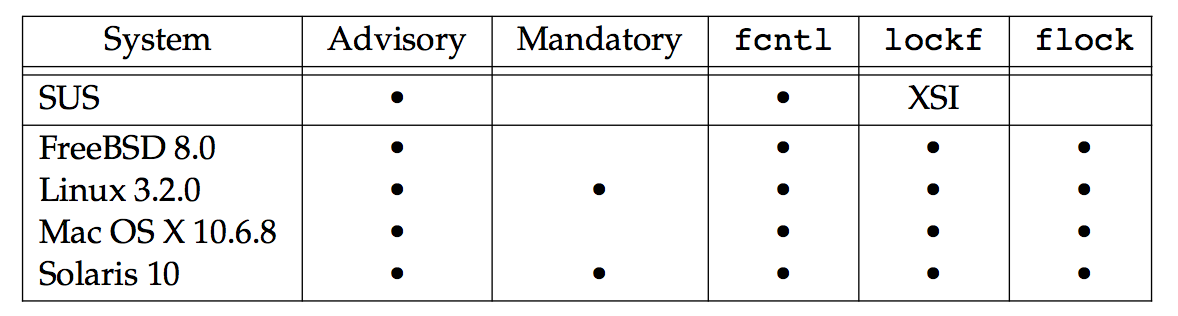
\includegraphics[width=0.8\linewidth]{figures/fig14_2-reclock.png}
    \caption{Forms of record locking supported by various \textsc{UNIX} systems}
  \end{figure}
\end{frame}


\begin{frame}[fragile,t]
  \frametitle{\texttt{fcntl} Record Locking}

Prototype for the \texttt{fcntl} function
\begin{codedef}
#include <fcntl.h>
int fcntl(int fd, int cmd, ... /* struct flock *flockptr */ );
// Returns: depends on cmd if OK (see following), −1 on error
\end{codedef}

\begin{itemize}
\item \textit{cmd}: \texttt{F\_GETLK}, \texttt{F\_SETLK}, \texttt{F\_SETLKW}
\item \textit{flockptr}: is a pointer to an \texttt{flock} structure
\end{itemize}

{\footnotesize
\begin{verbatim}
struct flock {
   short  l_type;   /* F_RDLCK, F_WRLCK, or F_UNLCK */
   short  l_whence; /* SEEK_SET, SEEK_CUR, or SEEK_END */
   off_t  l_start;  /* offset in bytes, relative to l_whence */
   off_t  l_len;    /* length, in bytes; 0 means lock to EOF */
   pid_t  l_pid;    /* returned with F_GETLK */
};
\end{verbatim}
}
\end{frame}

\begin{frame}[t]
  \frametitle{\texttt{fcntl} Record Locking cnt'd}
Rules in specification of the region to be locked or unlocked
\begin{itemize}
\item The two elements that specify the starting offset of the region are similar to the last two arguments of the \texttt{lseek} function.
  \begin{itemize}
  \item the \texttt{l\_whence} member is specified as
    \texttt{SEEK\_SET}, \texttt{SEEK\_CUR}, or \texttt{SEEK\_END}.
  \end{itemize}

\item  Locks can start and extend beyond the current end of file, but cannot start or extend before the beginning of the file.
\item  If \texttt{l\_len} is \texttt{0}, it means that the lock extends to the largest possible offset of the file.
\item To lock the entire file, we set \texttt{l\_start} and \texttt{l\_whence} to point to the beginning of the file and specify a length (\texttt{l\_len}) of \texttt{0}. {\footnotesize (There are several ways to specify the beginning of the file, but most applications specify \texttt{l\_start} as \texttt{0} and \texttt{l\_whence} as \texttt{SEEK\_SET}.)}
\end{itemize}
\end{frame}

\begin{frame}[t]
  \frametitle{\texttt{fcntl} Record Locking cnt'd}
The basic rule
\begin{itemize}
\item any number of processes can have a shared read lock on a given
  byte
\item only one process can have an exclusive write lock on a
  given byte.
\end{itemize}

\bigskip
Furthermore, if there are one or more read locks on a byte, there can’t be any write locks on that byte; 

\bigskip
if there is an exclusive write lock on a byte, there can’t be any read locks on that byte.  
\end{frame}

\begin{frame}[t]
  \frametitle{\texttt{fcntl} Record Locking cnt'd}

  \begin{figure}[h]
   \centering
    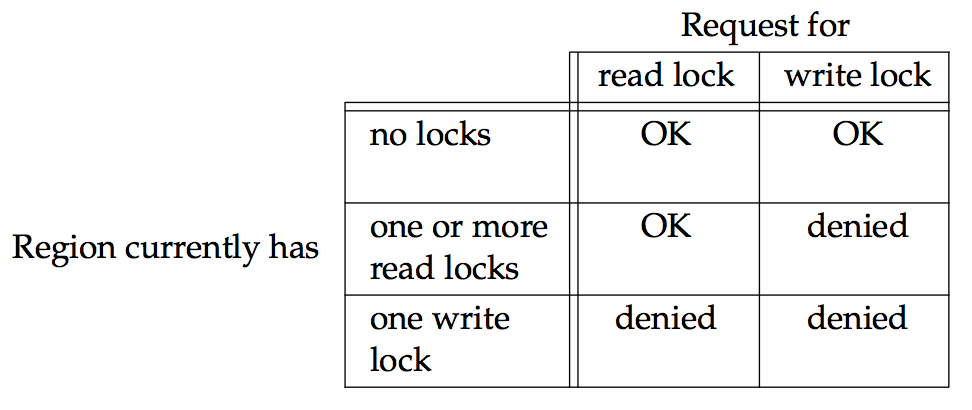
\includegraphics[width=0.7\linewidth]{figures/fig14_3-compatibility.png}
    \caption{Compatibility between different lock types}
  \end{figure}  

\bigskip

If a process has an existing lock on a range of a file, a subsequent attempt to place a lock on the same range by the same process \textbf{will replace the existing lock with the new one}. 
\end{frame}



\begin{frame}[t]
  \frametitle{\texttt{fcntl} Record Locking cnt'd}

Three commands for the \texttt{fcntl} function
  \begin{itemize}
  \item \texttt{F\_GETLK}: Determine whether the lock described by \textit{flockptr} is blocked by some other lock.
{\footnotesize
    \begin{itemize}
    \item If a lock exists, the information on that existing lock
      overwrites the information pointed to by \textit{flockptr}.
    \item If no lock exists, the structure pointed to by \textit{flockptr} is
      left unchanged except for the \texttt{l\_type} member, which is
      set to \texttt{F\_UNLCK}.
    \end{itemize}
}
  \item \texttt{F\_SETLK}:  Set the lock described by \textit{flockptr}.
{\footnotesize
    \begin{itemize}
    \item If the compatibility rule prevents the system from giving us
      the lock, \texttt{fcntl} returns immediately with errno set to
      either \texttt{EACCES} or \texttt{EAGAIN}.
    \end{itemize}
}
  \item \texttt{F\_SETLKW}: a blocking version of \texttt{F\_SETLK}.
{\footnotesize
    \begin{itemize}
    \item If the requested lock cannot be granted the calling process
      is put to sleep. The process wakes up either when the lock
      becomes available or when interrupted by a signal.
    \end{itemize}
}
  \end{itemize}
\end{frame}

\begin{frame}[t]
  \frametitle{\texttt{fcntl} Record Locking cnt'd}
Be aware that testing for a lock with \texttt{F\_GETLK} and then trying to obtain that lock with \texttt{F\_SETLK} or \texttt{F\_SETLKW} is not an atomic operation.

When setting or releasing a lock on a file, the system combines or splits adjacent areas as required.

  \begin{figure}[h]
   \centering
    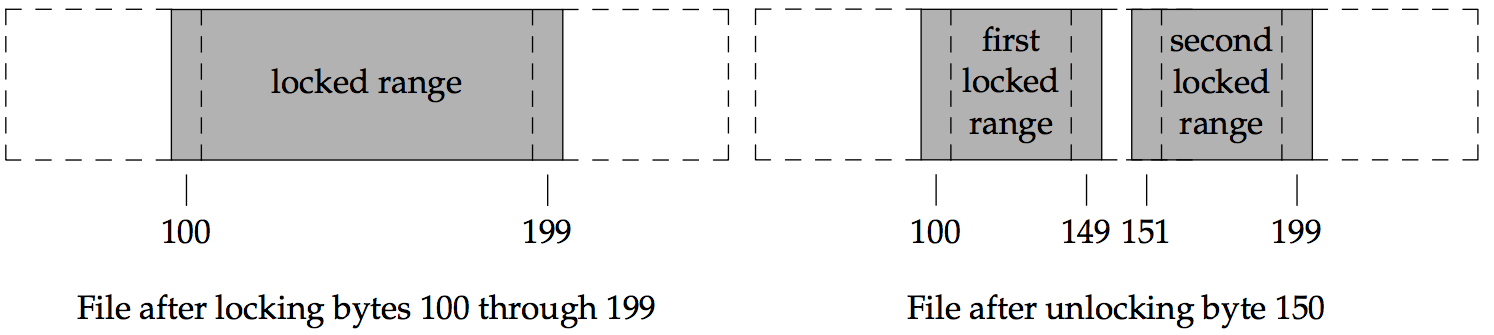
\includegraphics[width=1\linewidth]{figures/fig14_4-file.png}
    \caption{File byte-range lock diagram}
  \end{figure}
\end{frame}


\begin{frame}[t, fragile]





  \frametitle{Example: Requesting and Releasing a Lock}
Definition of \texttt{lock\_reg}

\begin{codedef}
#include <fcntl.h>
int
lock_reg(int fd, int cmd, int type, off_t offset, int whence, off_t len)
{
    struct flock    lock;
    lock.l_type = type;     /* F_RDLCK, F_WRLCK, F_UNLCK */
    lock.l_start = offset;  /* byte offset, relative to l_whence */
    lock.l_whence = whence; /* SEEK_SET, SEEK_CUR, SEEK_END */
    lock.l_len = len;       /* #bytes (0 means to EOF) */
    return(fcntl(fd, cmd, &lock));
}
\end{codedef}
\end{frame}

\begin{frame}[t, fragile]
  \frametitle{Example: Requesting and Releasing a Lock}
Use following five macros 
\begin{codedef}
#define	read_lock(fd, offset, whence, len) \
	lock_reg((fd), F_SETLK, F_RDLCK, (offset), (whence), (len))
#define	readw_lock(fd, offset, whence, len) \
	lock_reg((fd), F_SETLKW, F_RDLCK, (offset), (whence), (len))
#define	write_lock(fd, offset, whence, len) \
	lock_reg((fd), F_SETLK, F_WRLCK, (offset), (whence), (len))
#define	writew_lock(fd, offset, whence, len) \
	lock_reg((fd), F_SETLKW, F_WRLCK, (offset), (whence), (len))
#define	un_lock(fd, offset, whence, len) \
	lock_reg((fd), F_SETLK, F_UNLCK, (offset), (whence), (len))
\end{codedef}
\end{frame}

\begin{frame}[t, fragile, allowframebreaks]
  \frametitle{Example: Requesting and Releasing a Lock}
\begin{codedef}
#include <fcntl.h>
#include <stdlib.h>

pid_t lock_test(int fd, int type, off_t offset, int whence, off_t len)
{
    struct flock  lock;
    lock.l_type = type;		/* F_RDLCK or F_WRLCK */
    lock.l_start = offset;	/* byte offset, relative to l_whence */
    lock.l_whence = whence;	/* SEEK_SET, SEEK_CUR, SEEK_END */
    lock.l_len = len;		/* #bytes (0 means to EOF) */

    if (fcntl(fd, F_GETLK, &lock) < 0){
       fprintf(stderr, "fcntl error");
       exit(1);
    }

    if (lock.l_type == F_UNLCK)
       return(0);		/* false, region isn't locked by another proc */
       return(lock.l_pid);	/* true, return pid of lock owner */
}  
\end{codedef}
\end{frame}


\begin{frame}[t, fragile]
  \frametitle{Example: Requesting and Releasing a Lock}

  \begin{itemize}
  \item If a lock exists, this function returns the process ID of the
    process holding the lock.
  \item Otherwise, the function returns 0 (false).
  \end{itemize}

macros
\begin{codedef}
#define is_read_lockable(fd, offset, whence, len) \
        (lock_test((fd), F_RDLCK, (offset), (whence), (len)) == 0)
#define is_write_lockable(fd, offset, whence, len) \
        (lock_test((fd), F_WRLCK, (offset), (whence), (len)) == 0)
\end{codedef}

\end{frame}

\begin{frame}[t, fragile, allowframebreaks]
  \frametitle{Example: \texttt{codes/deadlock.c}}

\lstinputlisting[lineskip=0pt]{codes/deadlock.c}  
  
When a deadlock is detected, the kernel has to choose one process to receive the error return.

\begin{verbatim}
James@maker:codes$ ./deadlock
parent: got the lock, byte 1
child: got the lock, byte 0
child: writew_lock errorparent: got the lock, byte 0
\end{verbatim}
\end{frame}

\begin{frame}[fragile,t]
  \frametitle{implied Inheritence and Release of Locks}
Three rules govern the automatic inheritance and release of record locks  
\begin{itemize}
  \item Locks are associated with a process and a file. 
    \begin{itemize}
    \item when a process terminates, all its locks are released
    \item whenever a descriptor is closed, any locks on the file referenced by that descriptor for that process are released.
    \end{itemize}
\end{itemize}

\bigskip
Example

{\footnotesize
\begin{columns}[t]
  \begin{column}{0.5\textwidth}
After the \texttt{close(fd2)}, the lock on \texttt{fd1} is released
\begin{verbatim}
fd1 = open(pathname, ...);
read_lock(fd1, ...);
fd2 = dup(fd1);
close(fd2);
\end{verbatim}
  \end{column}
  \begin{column}{0.5\textwidth}
The same would happen if we replace \texttt{dup} with \texttt{open}
\begin{verbatim}
fd1 = open(pathname, ...);
read_lock(fd1, ...);
// if pathname is same
fd2 = open(pathname, ...); 
close(fd2);
\end{verbatim}    
  \end{column}
\end{columns}
}
\end{frame}


\begin{frame}[t]
  \frametitle{implied Inheritence and Release of Locks cnt'd}
Three rules govern the automatic inheritance and release of record locks  
\begin{itemize}
  \item Locks are associated with a process and a file.
  \item Locks are never inherited by the child across a \texttt{fork}.
    \begin{itemize}
    \item The child has to call \texttt{fcntl} to obtain its own locks on any
      descriptors that were inherited across the \texttt{fork}.
    \item locks are meant to prevent multiple
      processes from writing to the same file at the same time. 
    \end{itemize}

  \item Locks are inherited by a new program across an \texttt{exec}.
\end{itemize}
  
\end{frame}

\begin{frame}[fragile,t]
  \frametitle{FreeBSD Implementation}
To understand rule 1
\begin{verbatim}
fd1 = open(pathname, ...);
write_lock(fd1, 0, SEEK_SET, 1);
if ((pid = fork()) > 0) {
    fd2 = dup(fd1);
    fd3 = open(pathname, ...);
} else if (pid == 0) {
/* parent write locks byte 0 */
/* parent */
    read_lock(fd1, 1, SEEK_SET, 1); /* child read locks byte 1 */
}
pause();
\end{verbatim}
\end{frame}

\begin{frame}[t]
  \frametitle{FreeBSD Implementation cnt'd}
\begin{columns}[t]
  \begin{column}{0.4\textwidth}
{\footnotesize
    \begin{itemize}
    \item \texttt{lockf} structures that are linked together from the
      i-node structure
    \item Each \texttt{lockf} structure describes one locked region for a given process
    \item In the parent, closing any one of fd1, fd2, or fd3 causes the parent’s lock to be released. {\footnotesize When any one of these three file descriptors is closed, the kernel goes through the linked list of locks for the corresponding i-node and releases the locks held by the calling process.}
    \end{itemize}
}
  \end{column}
  \begin{column}{0.59\textwidth}
    \begin{figure}[h]
      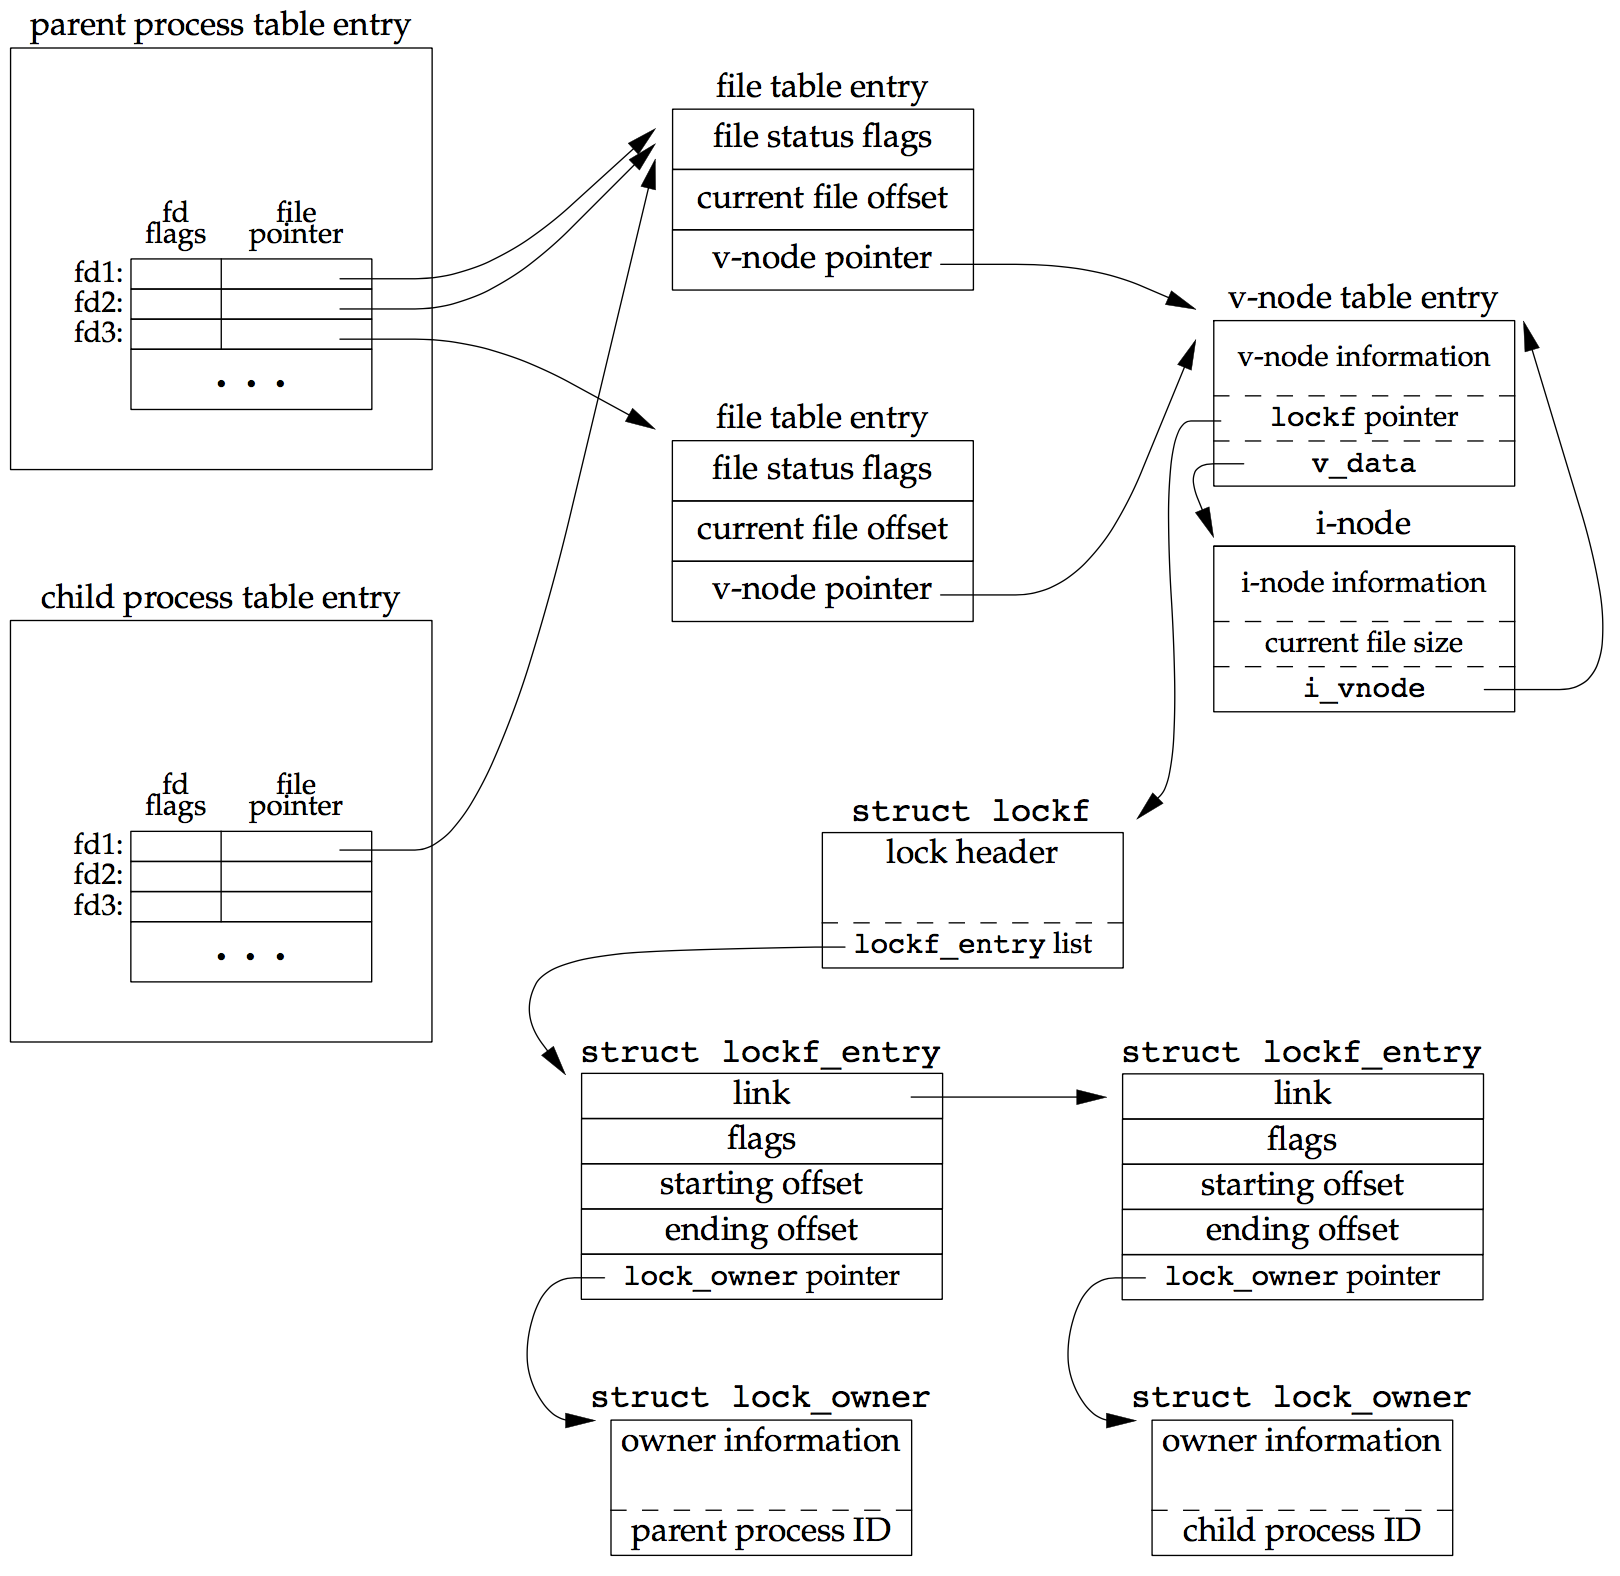
\includegraphics[width=1\linewidth]{figures/fig14_8-freebsd.png}
      \caption{The FreeBSD data structures for record locking}
    \end{figure}

  \end{column}

\end{columns}

\end{frame}


\begin{frame}[fragile,t]
  \frametitle{Locks at End of File}
We need to use caution when locking or unlocking byte ranges relative to the end of file.
\begin{itemize}
\item Most implementations convert an \texttt{l\_whence} value of \texttt{SEEK\_CUR} or \texttt{SEEK\_END} into an absolute file offset, using \texttt{l\_start} and the file’s current position or current length.
\end{itemize}
\begin{columns}[t]
  \begin{column}{0.41\textwidth}
    {\footnotesize
\begin{verbatim}
writew_lock(fd, 0, SEEK_END, 0);
write(fd, buf, 1);
un_lock(fd, 0, SEEK_END);
write(fd, buf, 1);
\end{verbatim}

The unlock operation that follows has the effect of removing the locks for future writes that append data to the file, but it leaves a lock on the last byte in the file.
    }
  \end{column}
  \begin{column}{0.59\textwidth}
    \begin{figure}[h]
      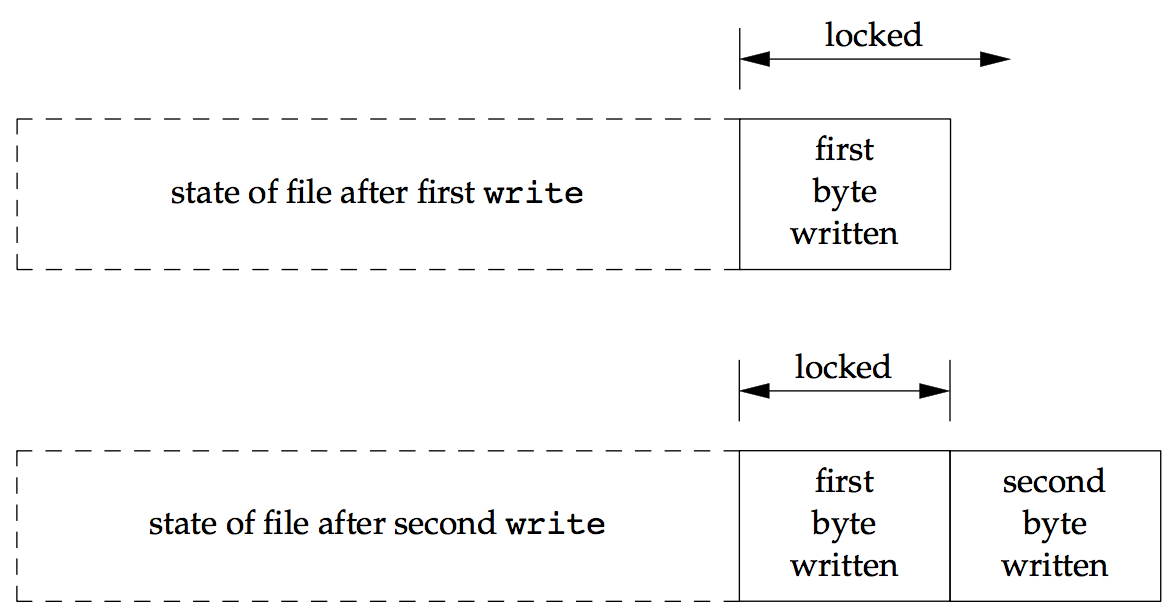
\includegraphics[width=1\linewidth]{figures/fig14_10-filerange.png}
      \caption{File range lock diagram}
    \end{figure}

  \end{column}

\end{columns}

\end{frame}

\begin{frame}[t]
  \frametitle{Advisory versus Mandatory Locking}
  \begin{block}{\textit{Cooperating processes}}
    If all the functions in the library handle record locking in a consistent way, then we say that any set of processes using these functions to access a database are \textit{cooperating processes}.
  \end{block}

It is feasible for these database access functions to use \textbf{advisory locking}, 
 if they are the only ones being used to access the database.
\bigskip

\textbf{Mandatory Locking} or \textit{enforcement-mode locking} causes the kernel to check \texttt{open}, \texttt{read}, \texttt{write} to verify that the calling process isn't violating a lock on the file being accessed
  

\end{frame}


\section{Asynchronous I/O}

\begin{frame}[t]
  \frametitle{Asynchronous I/O}
The cost of using Asynchronous I/O
\begin{itemize}
\item we complicate the design of our application by choosing to
  juggle multiple concurrent operations.
\item We have to worry about three sources of errors for every asynchronous operation
  \begin{itemize}
  \item one associated with the submission of the operation,
  \item one associated with the result of the operation itself,
  \item and one associated with the functions used to determine the
    status of the asynchronous operations.
  \end{itemize}
\item The interfaces themselves involve a lot of extra setup and processing rules compared to their conventional counterparts
\item Recovering from errors can be difficult.
\end{itemize}
  
\end{frame}


\begin{frame}[fragile,t]
  \frametitle{POSIX Asynchronous I/O}
The POSIX asynchronous I/O interfaces give us a consistent way to perform asynchronous I/O, regardless of the type of file.
\bigskip
The asynchronous I/O interfaces use AIO control blocks to describe I/O operations.

\begin{verbatim}
struct aiocb {
  int             aio_fildes;      /* file descriptor */
  off_t           aio_offset;      /* file offset fro I/O */
  volatile void  *aio_buf;         /* buffer for I/O */
  size_t          aio_nbytes;      /* number of bytes to transfer */
  int             aio_reqprio;     /* priority  */
  struct sigevent aio_sigevent;    /* Signal information  */
  int             aio_lio_opcode;  /* operation for list I/O */
};
\end{verbatim}
\end{frame}

\begin{frame}[fragile,t]
  \frametitle{POSIX Asynchronous I/O cnt'd}
The \texttt{aio\_sigevent} field controls how the application is notified about the completion of the I/O event.
{\footnotesize
\begin{verbatim}
struct sigevent {
     int   sigev_notify;           /* nofity type */
     int   sigev_signo;            /* signal number */
     union sigval  sigev value;    /* notify argument */
     void (*sigev_notify_function)(union sigval); /* notify function */
     pthread_attr_t *sigev_notify_attributes;     /* notify attrs */
};
\end{verbatim}

\texttt{sigev\_notify} field controls the type of notification
\begin{enumerate}
\item \texttt{SIGEV\_NONE}: The process is not notified when the asynchronous I/O request completes.
\item \texttt{SIGEV\_SIGNAL}: The signal specified by the \texttt{sigev\_signo} field is generated when the asynchronous I/O request completes. 
\item \texttt{SIGEV\_THREAD}: The function specified by the \texttt{sigev\_notify\_function} field is called when the asynchronous I/O request completes. The function is executed in a separate thread
\end{enumerate}
}
\end{frame}

\begin{frame}[t, fragile]
  \frametitle{POSIX Asynchronous I/O: Read and Write}
To perform asynchronous I/O, we need to initialize an AIO control block
\begin{codedef}
#include <aio.h>
int aio_read(struct aiocb *aiocb); int aio_write(struct aiocb *aiocb);
// Both return: 0 if OK, −1 on error
\end{codedef}
\bigskip
When these functions return success, 
\begin{itemize}
\item the asynchronous I/O request has been queued for processing by
  the operating system.
\end{itemize}
\bigskip

The return value bears no relation to the result of the actual I/O operation
\end{frame}


\begin{frame}[t, fragile]
  \frametitle{POSIX Asynchronous I/O: Persistency}
To force all pending asynchronous writes to persistent storage without waiting
\begin{codedef}
#include <aio.h>
int aio_fsync(int op, struct aiocb *aiocb);
// Returns: 0 if OK, −1 on error
\end{codedef}
The \texttt{aio\_fildes} field in the AIO control block indicates the file whose asynchronous writes are synched. 
\bigskip
If the \texttt{op} argument is set to
\begin{itemize}
\item \texttt{O\_DSYNC}: the operation behaves like a call to
  \texttt{fdatasync}.
\item \texttt{O\_SYNC}: the operation behaves like a call to \texttt{fsync}.
\end{itemize}

Returns when the synch is scheduled. The data won’t be persistent until the asynchronous synch completes. 
\end{frame}

\begin{frame}[t, fragile]
  \frametitle{POSIX Asynchronous I/O: Status}
To determine the completion status of an asynchronous read, write, or synch operation

\begin{codedef}
#include <aio.h>
int aio_error(const struct aiocb *aiocb);
Returns: 0, -1, EINPROGRESS, others
\end{codedef}

Four return types
\begin{itemize}
\item \texttt{0}: The asynchronous operation completed successfully.
\item \texttt{-1}: The call to \texttt{aio\_error} failed
\item \texttt{EINPROGRESS}: The asynchronous read, write, or synch is still pending
\item \textit{anything esle}: error code corresponding to the failed asynchronous operation.
\end{itemize}
\end{frame}

\begin{frame}[t, fragile]
  \frametitle{POSIX Asynchronous I/O: Success}
If the asynchronous operation succeeded, we can call the \texttt{aio\_retur}n function to get the asynchronous operation’s return value
\begin{codedef}
#include <aio.h>
ssize_t aio_return(const struct aiocb *aiocb);
// Returns: ...
\end{codedef}
\textbf{Until the asynchronous operation completes, we need to be careful to avoid calling the aio\_return function}
\begin{itemize}
\item Results undefined until the operation completes
\item call \texttt{ait\_return} only one time per asynchronous I/O operation
\end{itemize}
\end{frame}


\begin{frame}[t, fragile]
  \frametitle{POSIX Asynchronous I/O: suspend}

When we have completed the processing and find that we still have asynchronous operations outstanding, 
we can call the \texttt{aio\_suspend} function to block until an operation completes.

\begin{codedef}
#include <aio.h>
int aio_suspend(const struct aiocb *const list[], int nent,
                const struct timespec *timeout);
// Returns: 0 if OK, −1 on error
\end{codedef}

Three things cause \texttt{aio\_suspend} to return
{\footnotesize
\begin{itemize}
  \item \texttt{-1}: Interrupted by a signal, \texttt{errno} is set to
    \texttt{EINTR}
  \item \texttt{-1}: \textit{timeout} argument expires without any of the I/O operations completing, \texttt{errno} is set to \texttt{EAGAIN}
\item \texttt{0}: if any of the I/O operations complete
\end{itemize}
}
\textit{list}  is a pointer to an array of AIO control block

\textit{nent} indicates the number of entries in the array
\end{frame}

\begin{frame}[t, fragile]
  \frametitle{POSIX Asynchronous I/O: Cancel}
When we have pending asynchronous I/O operations that we no longer want to complete, we can attempt to cancel them with the \texttt{aio\_cancel} function.

\begin{codedef}
#include <aio.h>
int aio_cancel(int fd, /* file descriptor */
              struct aiocb *aiocb); /* NULL: all oustanding AIO */
// Returns: (see following)
\end{codedef}

Four return values
\begin{itemize}
\item \texttt{AIO\_ALLDONE}: All doen before attempt to cancel
\item \texttt{AIO\_CANCELED}: All are canceled
\item \texttt{AIO\_NOTCANCELED}: At least one of the requested opeartion could not be canceled
\item \texttt{-1}: Failed. Error code stored in \texttt{errno} 
\end{itemize}

\end{frame}

\begin{frame}[t, fragile]
  \frametitle{POSIX Asynchronous I/O: set of I/O requests}
 The \texttt{lio\_listio} function submits a set of I/O requests described by a list of AIO control blocks.
 \begin{codedef}
#include <aio.h>
int lio_listio(int mode, struct aiocb *restrict const list[restrict],
               int nent, struct sigevent *restrict sigev);
// Returns: 0 if OK, −1 on error
 \end{codedef}

 \begin{itemize}
 \item \texttt{mode}
   \begin{itemize}
   \item \texttt{LIO\_WAIT}: won't return until all I/Os in the list are complete (\texttt{sigev} is ingored)
   \item \texttt{LIO\_NOWAIT}: returns as soon as the I/O requests are queued. Process is notified asynchronously when all of the I/O operations complete
   \end{itemize}
 \item \texttt{sigev}: can be set to NULL if don't want to be notified
 \item \texttt{list}: list of AIO control blocks specifying the I/O operations to perform
 \item \texttt{nent}: number of elements in the array
 \end{itemize}

\end{frame}



\begin{frame}[t, fragile, allowframebreaks]
  \frametitle{Example: \texttt{codes/rot13a.c}}
  \lstinputlisting[lineskip=0pt]{codes/rot13a.c}  

\end{frame}


\begin{frame}[t, fragile, allowframebreaks]
  \frametitle{Example: \texttt{codes/rot13c2.c}}
  \lstinputlisting[lineskip=-4pt, basicstyle=\footnotesize]{codes/rot13c2.c}  

\end{frame}


\section{\texttt{readv} and \texttt{writev} Functions}

\begin{frame}[t, fragile]
  \frametitle{\texttt{readv} and \texttt{writev} Functions}
The \texttt{readv} and \texttt{writev} functions let us read into and write from multiple noncontiguous buffers in a single function call. These operations are called \textit{scatter read} and \textit{gather write}.
\begin{codedef}
#include <sys/uio.h>
ssize_t readv(int fd, const struct iovec *iov, int iovcnt); 
ssize_t writev(int fd, const struct iovec *iov, int iovcnt);
// Both return: number of bytes read or written, −1 on error
\end{codedef}

\texttt{iov} is a pointer to an array of \texttt{iovec} structures
{\footnotesize
\begin{verbatim}
struct iovec {
       void   *iov_base;  /* starting address of buffer */
       size_t  iov_len;   /* size of buffer */
};
\end{verbatim}
}

The number of elements in the \texttt{iov} array is specified \texttt{iovcnt}
\end{frame}

\begin{frame}[t]
  \frametitle{\texttt{readv} and \texttt{writev} Functions}
\begin{figure}[h]
  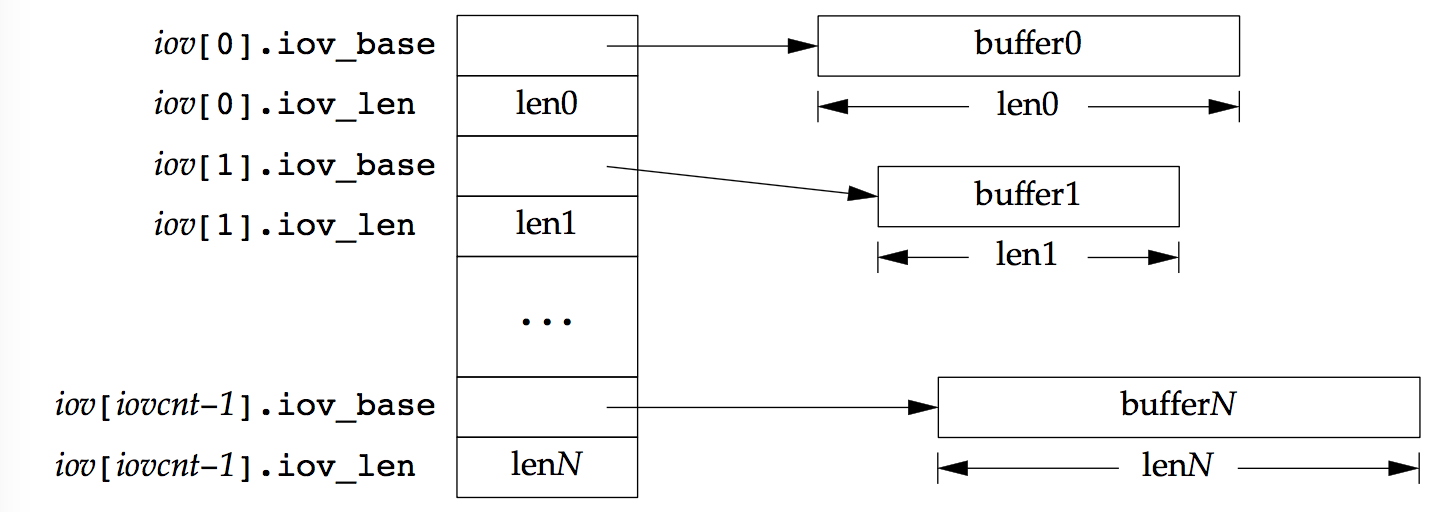
\includegraphics[width=0.8\linewidth]{figures/fig14_22-iovec.png}
  \caption{the \texttt{iovec} structure for \texttt{readv} and \texttt{writev}}
\end{figure}

{\footnotesize 
\begin{itemize}
\item The \texttt{writev} function gathers the output data from the buffers in order: \texttt{iov[0]}, \texttt{iov[1]}, through \texttt{iov[iovcnt−1]}
  \begin{itemize}
  \item \texttt{writev} returns the total number of bytes output,
    which should normally equal the sum of all the buffer lengths.
  \end{itemize}
\item The \texttt{readv} function scatters the data into the buffers in order, always filling one buffer before proceeding to the next.
  \begin{itemize}
  \item \texttt{readv} returns the total number of bytes that were
    read.
  \end{itemize}

\end{itemize}
}
\end{frame}



\section{\texttt{readn} and \texttt{writen} Functions}

\begin{frame}[t]
  \frametitle{\texttt{readn} and \texttt{writen} Functions}
Pipes, FIFOs, and some devices—notably terminals and networks—have the following
two properties.
\begin{enumerate}
\item A \texttt{read} operation may return less than asked for, even though we have not encountered the end of file.
  \begin{itemize}
  \item This is not an error, and we should simply continue reading from the device.
  \end{itemize}
\item A \texttt{write} operation can return less than we specified. This may be caused by kernel output buffers becoming full.
  \begin{itemize}
  \item it’s not an error, and we should continue writing the
    remainder of the data.
  \end{itemize}
Generally, when we read from or write to a pipe, network device, or terminal, we need to take these characteristics into consideration.
\end{enumerate}
\end{frame}

\begin{frame}[t, fragile]
  \frametitle{\texttt{readn} and \texttt{writen} Functions}
We can use the \texttt{readn} and \texttt{writen} functions to read and write \texttt{N} bytes of data, respectively, letting these functions handle a return value that’s possibly less than requested.  
\begin{itemize}
\item These two functions simply call read or write as many times as required to read or write the entire N bytes of data.
\end{itemize}
\begin{codedef}
ssize_t readn(int fd, void *buf, size_t nbytes); 
ssize_t writen(int fd, void *buf, size_t nbytes);
// Both return: number of bytes read or written, −1 on error
\end{codedef}
\end{frame}

\begin{frame}[t]
  \frametitle{\texttt{readn} Functions}
  \lstinputlisting[lineskip=0pt]{codes/readn.c}  

\end{frame}

\begin{frame}[t]
  \frametitle{\texttt{writen} Functions}
    \lstinputlisting[lineskip=0pt]{codes/writen.c}  

\end{frame}


\section{Memory-Mapped I/O}
\begin{frame}[t, fragile]
  \frametitle{Memory-Mapped I/O}
Memory-mapped I/O lets us map a file on disk into a buffer in memory so that, when we fetch bytes from the buffer, the corresponding bytes of the file are read.  
\bigskip
Similarly, when we store data in the buffer, the corresponding bytes are automatically written to the file. This lets us perform I/O without using \texttt{read} or \texttt{write}.


\end{frame}

\begin{frame}[t, fragile]
  \frametitle{Memory-Mapped I/O}

\begin{codedef}
#include <sys/mman.h>
void *mmap(void *addr, size_t len, int prot, int flag, int fd, off_t off );
// Returns: starting address of mapped region if OK, MAP_FAILED on error  
\end{codedef}
{\footnotesize
\begin{itemize}
\item \texttt{addr}: specify the address where we want the mapped region to start (Normally set to 0 to let system chooose)
\item \texttt{fd}: file descriptor specifying the file that is to be mapped (file must be opened before mapping)
\item \texttt{len}: number of bytes to map
\item \texttt{off}: starting offset in the file of the bytes to map
\item \texttt{prot}: READ, WRITE, and EXEC can be ORed
  \begin{itemize}
  \item \texttt{PROT\_READ}: Region can be read
  \item \texttt{PROT\_WRITE}: Region can be written
  \item \texttt{PROT\_EXEC}: Region can be executed
  \item \texttt{PROT\_NONE}: Region cannot be accessed
  \end{itemize}

\end{itemize}
}
\end{frame}

\begin{frame}[t]
  \frametitle{Memory-Mapped I/O}
\begin{figure}[h]
  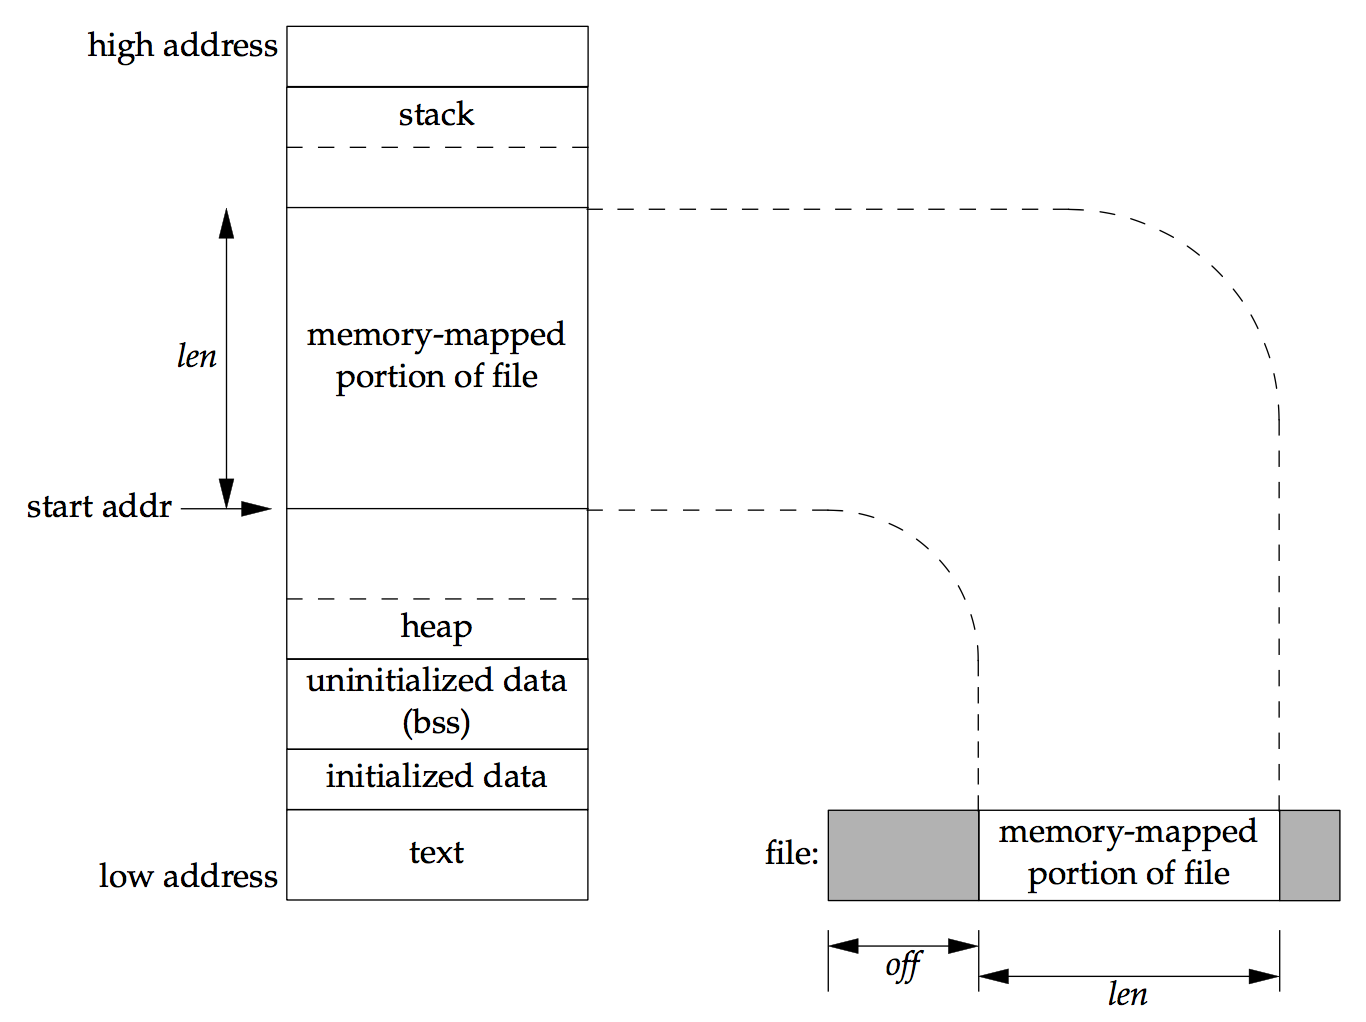
\includegraphics[width=0.8\linewidth]{figures/fig14_26-mmap.png}
  \caption{Example of a memory-mapped file}
\end{figure}

\end{frame}

\begin{frame}[t]
  \frametitle{Memory-Mapped I/O}
\texttt{flag} argument affects various attributes of the mapped region
\begin{itemize}
\item \texttt{MAP\_FIXED}: The return value must equal \texttt{addr}. Use of this flag is discouraged (Portability issue)
\item \texttt{MAP\_SHARED}: store operations into the mapped region by this process
\item \texttt{MAP\_PRIVATE}: store operation into the mapped region cause a private copy of the mapped file to be created. All successive references to the mapped region then reference the copy
\end{itemize}

\end{frame}

\begin{frame}[t]
  \frametitle{Memory-Mapped I/O}
\textbf{The value of \texttt{off} and the value of \texttt{addr} are usually required to be multiples of the system's virtual memory page size}
\bigskip
  What happens if the length of the mapped region isn't a multiple of the page size?
  \begin{itemize}
  \item File size 12 bytes
  \item Page size is 512 bytes
  \item system provides a mapped region of 512 bytes
  \item final 500 bytes of the this region are set to 0
  \item any changes to the final 500 bytes are not reflected to the file
  \end{itemize}
\end{frame}

\begin{frame}[t, fragile]
  \frametitle{Memory-Mapped I/O cnt'd}
 
  \begin{itemize}
  \item A memory-mapped region is inherited by a child across a \texttt{fork}
  \item But, is not inherited by the new program across an \texttt{exec}.
  \end{itemize}
\bigskip

Permission can be changed by calling \texttt{mprotect}
\begin{codedef}
#include <sys/mman.h>
int mprotect(void *addr, size_t len, int prot);
// Returns: 0 if OK, −1 on error
\end{codedef}

\end{frame}


\begin{frame}[t, fragile]
  \frametitle{Memory-Mapped I/O cnt'd}
When we modify pages that we’ve mapped into our address space using the \texttt{MAP\_SHARED} flag, the changes aren’t written back to the file immediately. 
\bigskip
kernel daemons decide when dirty pages are written back based on
\begin{itemize}
\item system load
\item configuration parameters meant to limit data loss in the event ofa system failure
\end{itemize}
\textbf{When the changes are written back, they are written in units of pages. }

\end{frame}


\begin{frame}[t, fragile]
  \frametitle{Memory-Mapped I/O cnt'd}
If the pages in a shared mapping have been modified, we can call \texttt{msync} to flush the changes to the file that backs the mapping. 
\begin{codedef}
#include <sys/mman.h>
int msync(void *addr, size_t len, int flags);
// Returns: 0 if OK, −1 on error  
\end{codedef}

Two values for \texttt{flags}
\begin{itemize}
\item \texttt{MS\_SYNC}: wait for the writes to complete before returning
\item \texttt{MS\_ASYNC}: simply schedule the pages to be written
\end{itemize}

\end{frame}


\begin{frame}[t, fragile]
  \frametitle{Memory-Mapped I/O cnt'd}
A memory-mapped region is automatically unmapped when the process terminates or we can unmap a region directly by calling the \texttt{munmap} function.
\begin{codedef}
#include <sys/mman.h>
int munmap(void *addr, size_t len);
// Returns: 0 if OK, −1 on error
\end{codedef}


\end{frame}


\begin{frame}[t, fragile, allowframebreaks]
  \frametitle{Example: CP with MMAP \texttt{codes/mcopy2.c}}
      \lstinputlisting[lineskip=0pt, basicstyle=\footnotesize]{codes/mcopy2.c}  

\texttt{dd if=/dev/urandom of=testfile count=1000000}

\texttt{time ./mcopy2 testfile mcopyout}

\texttt{time cp testfile mcopyout}
\end{frame}


%---------------------------------------------------------
\begin{comment}
\section{Last Words}

\begin{frame}[t]
  \frametitle{Last Words}

\begin{itemize}
\item 
\end{itemize}
\end{frame}

\end{comment}

\end{document}
